%% bare_jrnl.tex
%% V1.4b
%% 2015/08/26
%% by Michael Shell
%% see http://www.michaelshell.org/
%% for current contact information.
%%
%% This is a skeleton file demonstrating the use of IEEEtran.cls
%% (requires IEEEtran.cls version 1.8b or later) with an IEEE
%% journal paper.
%%
%% Support sites:
%% http://www.michaelshell.org/tex/ieeetran/
%% http://www.ctan.org/pkg/ieeetran
%% and
%% http://www.ieee.org/

%%*************************************************************************
%% Legal Notice:
%% This code is offered as-is without any warranty either expressed or
%% implied; without even the implied warranty of MERCHANTABILITY or
%% FITNESS FOR A PARTICULAR PURPOSE! 
%% User assumes all risk.
%% In no event shall the IEEE or any contributor to this code be liable for
%% any damages or losses, including, but not limited to, incidental,
%% consequential, or any other damages, resulting from the use or misuse
%% of any information contained here.
%%
%% All comments are the opinions of their respective authors and are not
%% necessarily endorsed by the IEEE.
%%
%% This work is distributed under the LaTeX Project Public License (LPPL)
%% ( http://www.latex-project.org/ ) version 1.3, and may be freely used,
%% distributed and modified. A copy of the LPPL, version 1.3, is included
%% in the base LaTeX documentation of all distributions of LaTeX released
%% 2003/12/01 or later.
%% Retain all contribution notices and credits.
%% ** Modified files should be clearly indicated as such, including  **
%% ** renaming them and changing author support contact information. **
%%*************************************************************************


% *** Authors should verify (and, if needed, correct) their LaTeX system  ***
% *** with the testflow diagnostic prior to trusting their LaTeX platform ***
% *** with production work. The IEEE's font choices and paper sizes can   ***
% *** trigger bugs that do not appear when using other class files.       ***                          ***
% The testflow support page is at:
% http://www.michaelshell.org/tex/testflow/



\documentclass[journal]{IEEEtran}
%
% If IEEEtran.cls has not been installed into the LaTeX system files,
% manually specify the path to it like:
% \documentclass[journal]{../sty/IEEEtran}





% Some very useful LaTeX packages include:
% (uncomment the ones you want to load)


% *** MISC UTILITY PACKAGES ***
%
%\usepackage{ifpdf}
% Heiko Oberdiek's ifpdf.sty is very useful if you need conditional
% compilation based on whether the output is pdf or dvi.
% usage:
% \ifpdf
%   % pdf code
% \else
%   % dvi code
% \fi
% The latest version of ifpdf.sty can be obtained from:
% http://www.ctan.org/pkg/ifpdf
% Also, note that IEEEtran.cls V1.7 and later provides a builtin
% \ifCLASSINFOpdf conditional that works the same way.
% When switching from latex to pdflatex and vice-versa, the compiler may
% have to be run twice to clear warning/error messages.






% *** CITATION PACKAGES ***
%
\usepackage{cite}
% cite.sty was written by Donald Arseneau
% V1.6 and later of IEEEtran pre-defines the format of the cite.sty package
% \cite{} output to follow that of the IEEE. Loading the cite package will
% result in citation numbers being automatically sorted and properly
% "compressed/ranged". e.g., [1], [9], [2], [7], [5], [6] without using
% cite.sty will become [1], [2], [5]--[7], [9] using cite.sty. cite.sty's
% \cite will automatically add leading space, if needed. Use cite.sty's
% noadjust option (cite.sty V3.8 and later) if you want to turn this off
% such as if a citation ever needs to be enclosed in parenthesis.
% cite.sty is already installed on most LaTeX systems. Be sure and use
% version 5.0 (2009-03-20) and later if using hyperref.sty.
% The latest version can be obtained at:
% http://www.ctan.org/pkg/cite
% The documentation is contained in the cite.sty file itself.






% *** GRAPHICS RELATED PACKAGES ***
%
\ifCLASSINFOpdf
  \usepackage[pdftex]{graphicx}
  % declare the path(s) where your graphic files are
  % \graphicspath{{../pdf/}{../jpeg/}}
  % and their extensions so you won't have to specify these with
  % every instance of \includegraphics
  % \DeclareGraphicsExtensions{.pdf,.jpeg,.png}
\else
  % or other class option (dvipsone, dvipdf, if not using dvips). graphicx
  % will default to the driver specified in the system graphics.cfg if no
  % driver is specified.
  % \usepackage[dvips]{graphicx}
  % declare the path(s) where your graphic files are
  % \graphicspath{{../eps/}}
  % and their extensions so you won't have to specify these with
  % every instance of \includegraphics
  % \DeclareGraphicsExtensions{.eps}
\fi
% graphicx was written by David Carlisle and Sebastian Rahtz. It is
% required if you want graphics, photos, etc. graphicx.sty is already
% installed on most LaTeX systems. The latest version and documentation
% can be obtained at: 
% http://www.ctan.org/pkg/graphicx
% Another good source of documentation is "Using Imported Graphics in
% LaTeX2e" by Keith Reckdahl which can be found at:
% http://www.ctan.org/pkg/epslatex
%
% latex, and pdflatex in dvi mode, support graphics in encapsulated
% postscript (.eps) format. pdflatex in pdf mode supports graphics
% in .pdf, .jpeg, .png and .mps (metapost) formats. Users should ensure
% that all non-photo figures use a vector format (.eps, .pdf, .mps) and
% not a bitmapped formats (.jpeg, .png). The IEEE frowns on bitmapped formats
% which can result in "jaggedy"/blurry rendering of lines and letters as
% well as large increases in file sizes.
%
% You can find documentation about the pdfTeX application at:
% http://www.tug.org/applications/pdftex





% *** MATH PACKAGES ***
%
\usepackage{amsmath}
% A popular package from the American Mathematical Society that provides
% many useful and powerful commands for dealing with mathematics.
%
% Note that the amsmath package sets \interdisplaylinepenalty to 10000
% thus preventing page breaks from occurring within multiline equations. Use:
%\interdisplaylinepenalty=2500
% after loading amsmath to restore such page breaks as IEEEtran.cls normally
% does. amsmath.sty is already installed on most LaTeX systems. The latest
% version and documentation can be obtained at:
% http://www.ctan.org/pkg/amsmath





% *** SPECIALIZED LIST PACKAGES ***
%
%\usepackage{algorithmic}
% algorithmic.sty was written by Peter Williams and Rogerio Brito.
% This package provides an algorithmic environment fo describing algorithms.
% You can use the algorithmic environment in-text or within a figure
% environment to provide for a floating algorithm. Do NOT use the algorithm
% floating environment provided by algorithm.sty (by the same authors) or
% algorithm2e.sty (by Christophe Fiorio) as the IEEE does not use dedicated
% algorithm float types and packages that provide these will not provide
% correct IEEE style captions. The latest version and documentation of
% algorithmic.sty can be obtained at:
% http://www.ctan.org/pkg/algorithms
% Also of interest may be the (relatively newer and more customizable)
% algorithmicx.sty package by Szasz Janos:
% http://www.ctan.org/pkg/algorithmicx




% *** ALIGNMENT PACKAGES ***
%
%\usepackage{array}
% Frank Mittelbach's and David Carlisle's array.sty patches and improves
% the standard LaTeX2e array and tabular environments to provide better
% appearance and additional user controls. As the default LaTeX2e table
% generation code is lacking to the point of almost being broken with
% respect to the quality of the end results, all users are strongly
% advised to use an enhanced (at the very least that provided by array.sty)
% set of table tools. array.sty is already installed on most systems. The
% latest version and documentation can be obtained at:
% http://www.ctan.org/pkg/array


% IEEEtran contains the IEEEeqnarray family of commands that can be used to
% generate multiline equations as well as matrices, tables, etc., of high
% quality.




% *** SUBFIGURE PACKAGES ***
%\ifCLASSOPTIONcompsoc
%  \usepackage[caption=false,font=normalsize,labelfont=sf,textfont=sf]{subfig}
%\else
%  \usepackage[caption=false,font=footnotesize]{subfig}
%\fi
% subfig.sty, written by Steven Douglas Cochran, is the modern replacement
% for subfigure.sty, the latter of which is no longer maintained and is
% incompatible with some LaTeX packages including fixltx2e. However,
% subfig.sty requires and automatically loads Axel Sommerfeldt's caption.sty
% which will override IEEEtran.cls' handling of captions and this will result
% in non-IEEE style figure/table captions. To prevent this problem, be sure
% and invoke subfig.sty's "caption=false" package option (available since
% subfig.sty version 1.3, 2005/06/28) as this is will preserve IEEEtran.cls
% handling of captions.
% Note that the Computer Society format requires a larger sans serif font
% than the serif footnote size font used in traditional IEEE formatting
% and thus the need to invoke different subfig.sty package options depending
% on whether compsoc mode has been enabled.
%
% The latest version and documentation of subfig.sty can be obtained at:
% http://www.ctan.org/pkg/subfig




% *** FLOAT PACKAGES ***
%
%\usepackage{fixltx2e}
% fixltx2e, the successor to the earlier fix2col.sty, was written by
% Frank Mittelbach and David Carlisle. This package corrects a few problems
% in the LaTeX2e kernel, the most notable of which is that in current
% LaTeX2e releases, the ordering of single and double column floats is not
% guaranteed to be preserved. Thus, an unpatched LaTeX2e can allow a
% single column figure to be placed prior to an earlier double column
% figure.
% Be aware that LaTeX2e kernels dated 2015 and later have fixltx2e.sty's
% corrections already built into the system in which case a warning will
% be issued if an attempt is made to load fixltx2e.sty as it is no longer
% needed.
% The latest version and documentation can be found at:
% http://www.ctan.org/pkg/fixltx2e


%\usepackage{stfloats}
% stfloats.sty was written by Sigitas Tolusis. This package gives LaTeX2e
% the ability to do double column floats at the bottom of the page as well
% as the top. (e.g., "\begin{figure*}[!b]" is not normally possible in
% LaTeX2e). It also provides a command:
%\fnbelowfloat
% to enable the placement of footnotes below bottom floats (the standard
% LaTeX2e kernel puts them above bottom floats). This is an invasive package
% which rewrites many portions of the LaTeX2e float routines. It may not work
% with other packages that modify the LaTeX2e float routines. The latest
% version and documentation can be obtained at:
% http://www.ctan.org/pkg/stfloats
% Do not use the stfloats baselinefloat ability as the IEEE does not allow
% \baselineskip to stretch. Authors submitting work to the IEEE should note
% that the IEEE rarely uses double column equations and that authors should try
% to avoid such use. Do not be tempted to use the cuted.sty or midfloat.sty
% packages (also by Sigitas Tolusis) as the IEEE does not format its papers in
% such ways.
% Do not attempt to use stfloats with fixltx2e as they are incompatible.
% Instead, use Morten Hogholm'a dblfloatfix which combines the features
% of both fixltx2e and stfloats:
%
% \usepackage{dblfloatfix}
% The latest version can be found at:
% http://www.ctan.org/pkg/dblfloatfix




%\ifCLASSOPTIONcaptionsoff
%  \usepackage[nomarkers]{endfloat}
% \let\MYoriglatexcaption\caption
% \renewcommand{\caption}[2][\relax]{\MYoriglatexcaption[#2]{#2}}
%\fi
% endfloat.sty was written by James Darrell McCauley, Jeff Goldberg and 
% Axel Sommerfeldt. This package may be useful when used in conjunction with 
% IEEEtran.cls'  captionsoff option. Some IEEE journals/societies require that
% submissions have lists of figures/tables at the end of the paper and that
% figures/tables without any captions are placed on a page by themselves at
% the end of the document. If needed, the draftcls IEEEtran class option or
% \CLASSINPUTbaselinestretch interface can be used to increase the line
% spacing as well. Be sure and use the nomarkers option of endfloat to
% prevent endfloat from "marking" where the figures would have been placed
% in the text. The two hack lines of code above are a slight modification of
% that suggested by in the endfloat docs (section 8.4.1) to ensure that
% the full captions always appear in the list of figures/tables - even if
% the user used the short optional argument of \caption[]{}.
% IEEE papers do not typically make use of \caption[]'s optional argument,
% so this should not be an issue. A similar trick can be used to disable
% captions of packages such as subfig.sty that lack options to turn off
% the subcaptions:
% For subfig.sty:
% \let\MYorigsubfloat\subfloat
% \renewcommand{\subfloat}[2][\relax]{\MYorigsubfloat[]{#2}}
% However, the above trick will not work if both optional arguments of
% the \subfloat command are used. Furthermore, there needs to be a
% description of each subfigure *somewhere* and endfloat does not add
% subfigure captions to its list of figures. Thus, the best approach is to
% avoid the use of subfigure captions (many IEEE journals avoid them anyway)
% and instead reference/explain all the subfigures within the main caption.
% The latest version of endfloat.sty and its documentation can obtained at:
% http://www.ctan.org/pkg/endfloat
%
% The IEEEtran \ifCLASSOPTIONcaptionsoff conditional can also be used
% later in the document, say, to conditionally put the References on a 
% page by themselves.




% *** PDF, URL AND HYPERLINK PACKAGES ***
%
%\usepackage{url}
% url.sty was written by Donald Arseneau. It provides better support for
% handling and breaking URLs. url.sty is already installed on most LaTeX
% systems. The latest version and documentation can be obtained at:
% http://www.ctan.org/pkg/url
% Basically, \url{my_url_here}.




% *** Do not adjust lengths that control margins, column widths, etc. ***
% *** Do not use packages that alter fonts (such as pslatex).         ***
% There should be no need to do such things with IEEEtran.cls V1.6 and later.
% (Unless specifically asked to do so by the journal or conference you plan
% to submit to, of course. )


% correct bad hyphenation here
\hyphenation{op-tical net-works semi-conduc-tor}


\begin{document}
%
% paper title
% Titles are generally capitalized except for words such as a, an, and, as,
% at, but, by, for, in, nor, of, on, or, the, to and up, which are usually
% not capitalized unless they are the first or last word of the title.
% Linebreaks \\ can be used within to get better formatting as desired.
% Do not put math or special symbols in the title.
\title{Role-Aware Multimodal Student Engagement Recognition for Online Collaborative Learning}
%
%
% author names and IEEE memberships
% note positions of commas and nonbreaking spaces ( ~ ) LaTeX will not break
% a structure at a ~ so this keeps an author's name from being broken across
% two lines.
% use \thanks{} to gain access to the first footnote area
% a separate \thanks must be used for each paragraph as LaTeX2e's \thanks
% was not built to handle multiple paragraphs
%

\author{Name%
% Add final affiliation, email addresses, and manuscript dates here if required
% by the target IEEE venue.
}

% note the % following the last \IEEEmembership and also \thanks - 
% these prevent an unwanted space from occurring between the last author name
% and the end of the author line. i.e., if you had this:
% 
% \author{....lastname \thanks{...} \thanks{...} }
%                     ^------------^------------^----Do not want these spaces!
%
% a space would be appended to the last name and could cause every name on that
% line to be shifted left slightly. This is one of those "LaTeX things". For
% instance, "\textbf{A} \textbf{B}" will typeset as "A B" not "AB". To get
% "AB" then you have to do: "\textbf{A}\textbf{B}"
% \thanks is no different in this regard, so shield the last } of each \thanks
% that ends a line with a % and do not let a space in before the next \thanks.
% Spaces after \IEEEmembership other than the last one are OK (and needed) as
% you are supposed to have spaces between the names. For what it is worth,
% this is a minor point as most people would not even notice if the said evil
% space somehow managed to creep in.



% The paper headers
\markboth{IEEE Journal Draft}%
{Gupta and Ghose: Role-Aware Multimodal Student Engagement Recognition}
% The only time the second header will appear is for the odd numbered pages
% after the title page when using the twoside option.
% 
% *** Note that you probably will NOT want to include the author's ***
% *** name in the headers of peer review papers.                   ***
% You can use \ifCLASSOPTIONpeerreview for conditional compilation here if
% you desire.




% If you want to put a publisher's ID mark on the page you can do it like
% this:
%\IEEEpubid{0000--0000/00\$00.00~\copyright~2015 IEEE}
% Remember, if you use this you must call \IEEEpubidadjcol in the second
% column for its text to clear the IEEEpubid mark.



% use for special paper notices
%\IEEEspecialpapernotice{(Invited Paper)}




% make the title area
\maketitle 

% As a general rule, do not put math, special symbols or citations
% in the abstract or keywords.
% As a general rule, do not put math, special symbols or citations
% in the abstract or keywords.
\begin{abstract}
Automatic student engagement recognition can help instructors understand when students are attentive, partially engaged, or disengaged during online learning. However, engagement is difficult to measure because it is expressed through several forms of behavior rather than through a single video frame or facial expression. Existing engagement systems often rely mainly on visual behavior and may not fully use audio information or the ordered structure of engagement labels. This is important because engagement datasets commonly represent student state as a scale, such as highly disengaged, disengaged, engaged, and highly engaged. In this paper, we propose a multimodal audio-video framework for online student engagement recognition. The model combines facial and visual behavior with speech-related audio features, then uses audio-video attention to learn how both modalities support the final engagement prediction. The proposed direction is motivated by recent engagement datasets, including DAiSEE, EngageNet, CMOSE, and COLER, where distinguishing between disengaged and engaged levels remains challenging. This paper focuses on a practical architecture for improving engagement recognition by combining visual behavior and audio participation while treating engagement as an ordered learning state.
\end{abstract}

% Note that keywords are not normally used for peerreview papers.
\begin{IEEEkeywords}
Student engagement, multimodal learning, online education, audio-visual fusion, ordinal classification.
\end{IEEEkeywords}






% For peer review papers, you can put extra information on the cover
% page as needed:
% \ifCLASSOPTIONpeerreview
% \begin{center} \bfseries EDICS Category: 3-BBND \end{center}
% \fi
%
% For peerreview papers, this IEEEtran command inserts a page break and
% creates the second title. It will be ignored for other modes.
\IEEEpeerreviewmaketitle



\section{Introduction}

\IEEEPARstart{S}{tudent} engagement is a key indicator of learning quality in online and hybrid classrooms. An engaged student is not only present in a session, but is also attentive, responsive, and involved in the learning activity. In face-to-face teaching, instructors judge this state by observing several forms of behavior together, including facial expression, posture, eye contact, speech, and interaction with classmates. In online learning, these signals become harder to interpret because students appear through webcams, microphones may be muted, and the instructor has limited access to the full classroom environment. For this reason, automatic student engagement recognition has become an important problem in educational technology and affective computing \cite{qarbal2025review}.

The main difficulty is that engagement is not expressed through one modality or one fixed behavior. Many engagement-recognition methods rely heavily on visual information such as face images, head pose, gaze direction, and facial action units. These features can capture visible attention, but they may not fully represent a student's learning state. A student may look at the screen without actively following the lesson, while another student may look away briefly while thinking. Audio can provide additional evidence through speaking activity, hesitation, tone, and participation patterns. However, existing online engagement datasets often contain limited or uneven speech, which makes audio difficult to use consistently. As a result, the boundary between disengaged and engaged states remains challenging, especially when both attentive listening and passive disengagement appear visually quiet \cite{singh2023engagenet,wu2024cmose}.

To address this problem, this paper develops a multimodal audio-video framework for online student engagement recognition. The visual branch extracts facial and temporal behavior from video frames, while the audio branch extracts speech-related information from the corresponding audio signal. The two streams are combined through an audio-video attention mechanism inspired by cross-attention methods used in multimodal emotion recognition \cite{venkatraman2025avtca}. This design allows the model to learn complementary information from both modalities instead of depending only on a single visual stream. The framework also treats engagement as an ordered learning state because datasets commonly describe engagement using levels such as highly disengaged, disengaged, engaged, and highly engaged \cite{wu2024cmose,tran2026ordinal}.

The experimental direction of this work focuses on evaluating whether audio-video fusion improves engagement recognition compared with vision-dominant baselines. In addition to standard classification metrics, the evaluation includes ordered-label measures such as adjacent accuracy and mean absolute class error. These metrics are important because they show not only whether the model predicts the exact class, but also how far the prediction is from the true engagement level. This is especially useful for analyzing errors between nearby classes, where the distinction is often subtle.

This paper claims that online student engagement recognition should be modeled as a multimodal and ordered-state prediction problem. By combining visual behavior, speech-related audio information, and engagement-aware evaluation, the proposed framework aims to provide a more reliable approach for recognizing engagement levels in online learning settings. The broader goal is to move toward systems that better match how instructors interpret students in real classrooms: by considering multiple behaviors together over time rather than relying on a single visible signal.

\section{Related Work}

\subsection{Student Engagement Recognition}

Student engagement recognition has been studied using computer vision, machine learning, and multimodal learning methods. Traditional engagement assessment often depends on instructor observation, self-report surveys, or manual coding. Although these methods can provide useful information, they are difficult to scale and may be subjective. For this reason, recent research has focused on automatic engagement detection using video, audio, behavior logs, and classroom interaction data \cite{qarbal2025review,theophilus2026review}. A recent review of 48 studies on learner engagement prediction reports that the great majority rely on hand-crafted or deep visual features from a single modality, and identifies feature engineering and dataset quality, rather than classifier choice, as the limiting factors \cite{theophilus2026review}.

Many early systems used visual features because face and body behavior are easy to capture from classroom or webcam videos. Common visual cues include facial expression, eye gaze, head pose, posture, and facial action units. These features can provide strong signals of attention and participation. However, vision-only systems also have limitations. They can be affected by lighting, camera angle, occlusion, and individual differences in expression. More importantly, visible attention is not always the same as cognitive engagement. A student may appear focused but not be mentally involved, while another student may look away briefly while thinking.

DAiSEE is one of the commonly used datasets for engagement recognition in online learning. It provides video clips labeled with engagement-related states and has been used to test several baseline models \cite{gupta2016daisee}. However, DAiSEE also shows common challenges in this area, including class imbalance, short clip-based labeling, and difficulty in judging internal student states from video alone. These issues make it difficult for models trained on one dataset to generalize well to real classroom settings. Class imbalance in particular has motivated dedicated remedies: generative augmentation of the under-represented low-engagement classes on EngageNet improves macro-F1 without a loss in overall accuracy \cite{yulius2025gan}, which indicates that minority-level performance is a distinct problem from headline accuracy.

EngageNet extends this direction by providing a larger engagement dataset collected in more diverse conditions \cite{singh2023engagenet}. It includes participants under different illumination and recording settings and evaluates features such as action units, gaze, head pose, and learned visual representations. The results show that engagement prediction remains challenging even with larger datasets, especially when the model must handle real-world variation. This supports the need for robust multimodal models rather than relying only on one type of visual cue. Along the same line, MSC-Trans fuses several visual feature groups through a transformer encoding structure and shows that fixed feature combinations limit classroom engagement detection \cite{xie2025msctrans}, and GLP-fusion combines global facial, local key-point and physiological features hierarchically to improve robustness against occlusion \cite{qin2026glpfusion}.

CMOSE further highlights the importance of label quality and multimodal information for online student engagement recognition \cite{wu2024cmose}. It addresses problems such as poor label quality, class imbalance, and large variation within the same engagement class. CMOSE also shows that speech and audio features can improve engagement prediction when they are available. This is important for online collaborative learning because participation is not only visual; it is also expressed through speaking behavior, hesitation, tone, and interaction. A recent framework that integrates visual, audio, physiological and behavior-log streams with a bidirectional LSTM reports that multimodal fusion outperforms vision-only and late-fusion baselines on CMOSE by a clear macro-F1 margin \cite{dan2026multimodal}, again pointing to the under-represented levels as the place where additional modalities pay off.

\subsection{Multimodal Audio-Visual Learning}

Multimodal learning is useful because human behavior is naturally expressed through more than one channel. In affective computing and emotion recognition, audio provides information about tone, intensity, rhythm, and hesitation, while video provides information about facial expression, movement, and visual attention. Combining these modalities can make the model more reliable than using only one source. Surveys of multimodal emotion recognition organise the field by fusion level and by how a model behaves when one modality is missing or weak \cite{li2025mersurvey}, which is precisely the situation in online classrooms where microphones are frequently muted. Deep convolutional and recurrent fusion of face and speech remains a strong and widely used baseline for audio-visual emotion recognition \cite{taware2025mer}, and comparable cross-modal architectures have been applied to sentiment polarity detection \cite{hegde2025sentiment} and to depression recognition from audio, video and text \cite{lu2026dstc}, where the DSTC network explicitly models modality differences before fusion.

Audio-video fusion has been widely studied in multimodal emotion recognition. AVT-CA uses transformer-based cross-attention to combine audio and visual information \cite{venkatraman2025avtca}. In this type of model, audio features can attend to visual features, and visual features can attend to audio features. This is useful because it allows the model to learn which parts of one modality support or correct the other modality. For student engagement recognition, this idea is helpful because audio and video may not always be equally reliable. For example, video may be unclear due to lighting or face occlusion, while audio may be missing or weak when students are silent.

Recent audio-visual fusion work also shows that the level of fusion matters. Some methods use late fusion, where separate audio and visual predictions are combined near the end. Other methods use early fusion, where audio and visual tokens interact earlier in the model. Early fusion can capture fine-grained relationships, but it may require more data and computation \cite{mo2024earlyfusion}. Attention bottleneck methods try to reduce unnecessary cross-modal interaction while still keeping the most useful information \cite{nagrani2021attention}. Transformer fusion of audio and visual streams has also been shown to improve action recognition over either modality alone, provided the two streams are brought to a common temporal resolution before they interact \cite{kim2024avaction}, a requirement that we address directly in our alignment module. These studies suggest that a practical engagement-recognition system should use multimodal fusion carefully instead of adding complexity without a clear reason.

\subsection{Ordinal and Context-Aware Engagement Modeling}

Engagement labels are usually ordered. For example, a four-level engagement scale may include highly disengaged, disengaged, engaged, and highly engaged. Treating these labels as unrelated classes ignores the natural order between them. A prediction error between engaged and highly engaged should not be treated the same as an error between highly disengaged and highly engaged. Therefore, ordinal modeling is important for engagement recognition.

Recent work has started to address this issue. CMOSE proposes a training strategy that considers the ordinal pattern of engagement levels \cite{wu2024cmose}. CORE-Net also uses ordinal supervision and context modeling for collaborative learning \cite{tran2026ordinal}. These studies show that engagement should not be modeled only as a standard classification problem. Instead, the model should understand both the order of labels and the classroom context in which behavior occurs.

Context is especially important in collaborative learning. Student engagement does not depend only on one student's face or voice. It is also influenced by the learning activity, group interaction, and the student's role in the conversation. A behavior that appears disengaged in one context may be normal or even productive in another context. For example, silence can indicate disengagement when a student is expected to speak, but it can also indicate active listening when another student is speaking.

Some recent models use richer context and hierarchical fusion to improve engagement prediction. GLP-fusion combines global facial features, local key-point features, and physiological features through a hierarchical fusion strategy \cite{qin2026glpfusion}. CORE-Net models group-level context for collaborative learning \cite{tran2026ordinal}. These methods show that engagement recognition benefits from information beyond a single facial frame. However, most existing models still do not directly treat speaker-listener role as a central part of the prediction process.

\subsection{Research Gap}

The reviewed studies show important progress in student engagement recognition, but several gaps remain. First, many models still depend mainly on visual information, even though audio and speech behavior can provide useful evidence of participation and confusion. Second, engagement is often treated as a flat class label, even though engagement levels are ordered. Third, current systems rarely model the student's conversational role. In collaborative learning, the same gaze, silence, or speech pattern can have different meanings depending on whether the student is speaking or listening.

This paper addresses these gaps by proposing a role-aware multimodal engagement-recognition framework. The proposed model combines audio-video fusion, ordinal engagement prediction, and speaker-listener role conditioning. This design is intended to be closer to how instructors judge engagement in real classrooms: by observing the student, listening to participation, and interpreting both signals within the learning context.



\section{Proposed Research Method}

We separate the proposed architecture into four components: A) an audio encoder, B) a visual encoder with a behavior feature stream, C) a temporal alignment and two-stage cross-attention fusion module, and D) an ordinal prediction head with calibrated decoding. We explain each component in the following subsections. The graphical representation of the complete architecture is presented in Fig.~\ref{fig_arch}.

% TODO (P6): draw.io architecture diagram -> figures/architecture.pdf
%\begin{figure*}[!t]
%\centering
%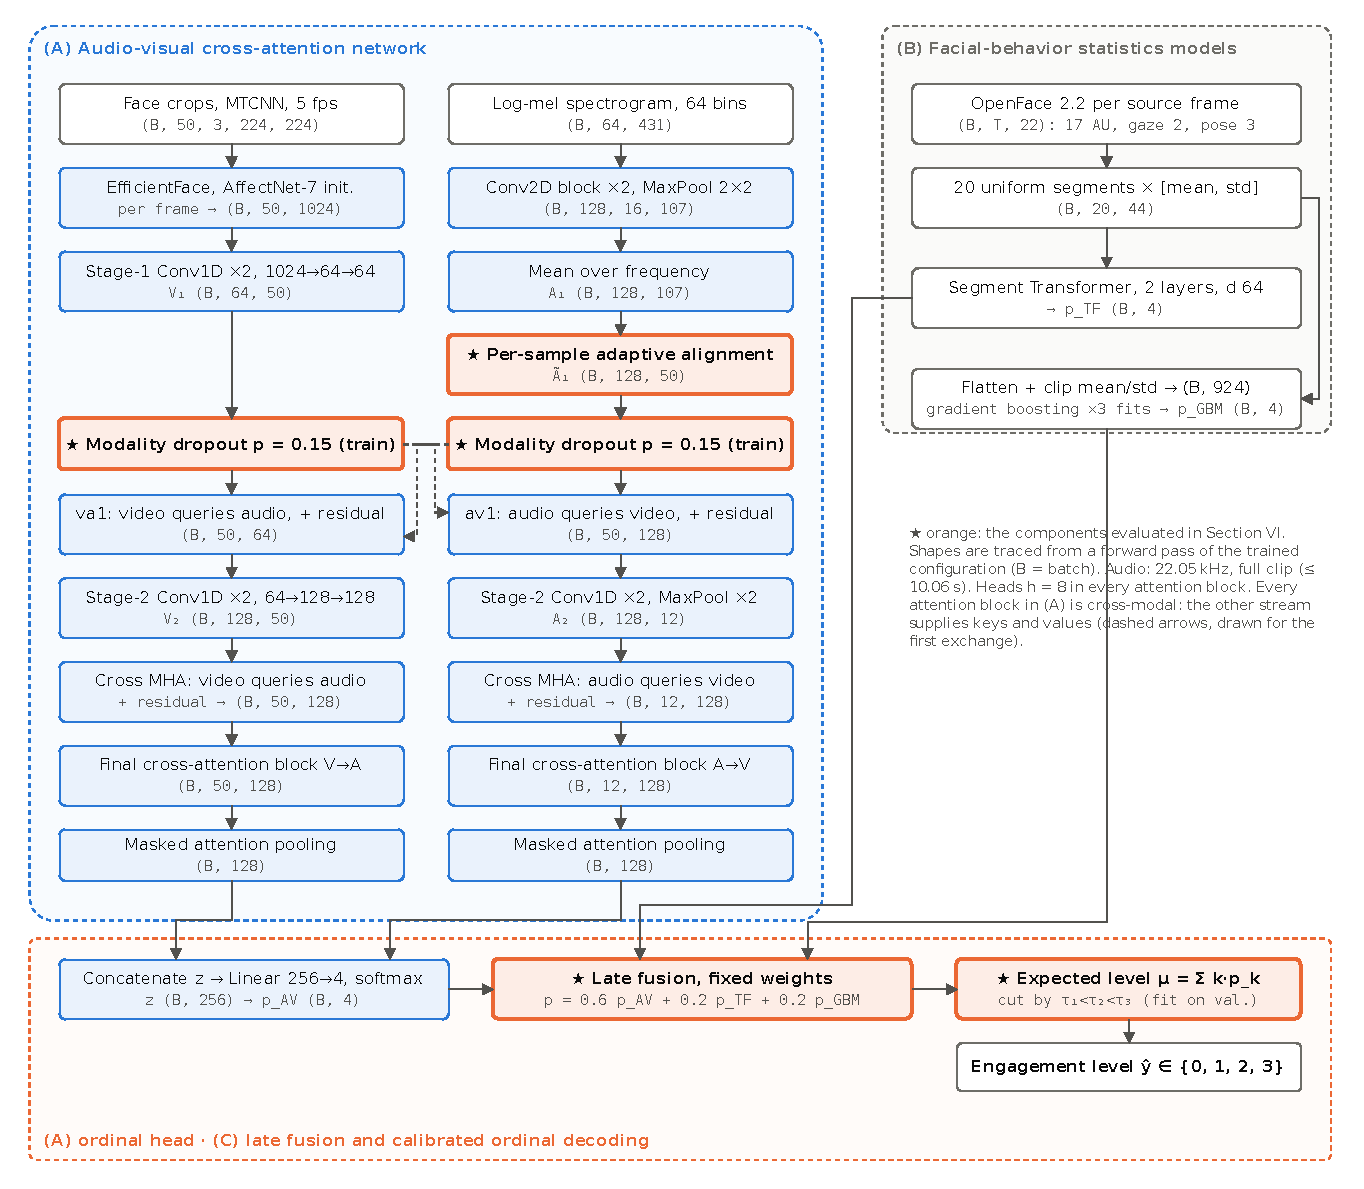
\includegraphics[width=6.5in]{figures/architecture}
%\caption{Overview of the proposed audio-visual engagement recognition architecture. Audio tokens are pooled onto the visual time axis before the first cross-attention block; the behavior stream provides facial action unit, gaze, and head-pose tokens; the ordinal head produces four logits that are decoded with validation-fitted thresholds.}
%\label{fig_arch}
%\end{figure*}

\subsection{Audio Encoder}

The audio branch receives the full 10\,s waveform of each clip, resampled to 22.05\,kHz and converted to a 64-bin log-mel spectrogram $\mathbf{X}_a \in \mathbb{R}^{64 \times T_a}$. A two-dimensional convolutional stack operates jointly over the frequency and time axes, after which the frequency axis is collapsed by averaging, producing a sequence of 128-dimensional temporal tokens at one quarter of the input frame rate. This sequence is the first-stage audio representation $\mathbf{A}_1 \in \mathbb{R}^{128 \times T_a/4}$. A second stage of two one-dimensional convolutions (128$\to$256$\to$128 channels) is applied after the first cross-attention exchange and yields $\mathbf{A}_2$. Mel-spectrogram input was preferred to MFCC features because the convolutional front end can learn its own frequency pooling, and because the 64-bin representation preserves the prosodic contours (pitch movement, energy envelope) that carry speaking activity and hesitation information.

\subsection{Visual Encoder and Behavior Stream}

\subsubsection{Visual Frame Encoder}
Each clip is sampled at 5 frames per second, giving up to 50 face crops of $224 \times 224$ pixels detected with MTCNN. Every frame is encoded independently by an EfficientFace backbone \cite{zhao2021efficientface} composed of inverted-residual blocks with a channel-and-spatial modulator, initialised from weights pre-trained on AffectNet-7. The backbone maps each frame to a 1024-dimensional embedding. The per-frame embeddings are stacked along time and passed through two one-dimensional convolutions (1024$\to$64$\to$64) that model short-range temporal dynamics, producing the first-stage visual token sequence $\mathbf{V}_1 \in \mathbb{R}^{64 \times T_v}$ with $T_v \le 50$. A second convolutional stage (64$\to$128$\to$128) produces $\mathbf{V}_2$.

\subsubsection{Behavior Feature Stream}
In addition to the learned frame embeddings, we extract an explicit behavior descriptor per frame with OpenFace \cite{baltrusaitis2018openface}: 17 facial action unit intensities, two gaze angles, and three head-pose rotations, giving a 22-channel sequence $\mathbf{B} \in \mathbb{R}^{22 \times T_v}$. Each channel is normalised by subtracting the subject-level mean so that the model observes deviations from a student's own resting behavior rather than absolute values. The sequence is encoded by a one-dimensional convolution (22$\to$128) followed by a bidirectional GRU, giving behavior tokens $\mathbf{H}_b \in \mathbb{R}^{128 \times T_v}$ and a mean-pooled summary $\mathbf{h}_b$. The audio-visual summary attends over $\mathbf{H}_b$ with a single cross-attention layer, and the pooled summary is added through a skip connection. When OpenFace fails to detect a face for a clip, the stream is replaced by a learned missing-modality token so that the fusion layer never receives silent zeros. The motivation for this stream is that action units, gaze, and head pose are the features on which the strongest published EngageNet baselines operate \cite{singh2023engagenet}, and explicit features are known to outperform end-to-end frame encoders on datasets of this size.

% Akshit's visual-emphasis variant — commented out until a matched number exists (plan.md §18.4).
%\subsubsection{Visual-Weighted Fusion Variant}
%Because most EngageNet clips contain no speech, we also evaluate a variant in which the visual summary receives a larger weight at the fusion point. This variant is corpus-specific; the equal-contribution design is retained for speech-rich classroom data.

\subsection{Temporal Alignment and Two-Stage Cross-Attention Fusion}

\subsubsection{Per-Sample Temporal Alignment}
After the first convolutional stage the audio sequence contains roughly 168 time steps for a 10\,s clip whereas the visual sequence contains at most 50. If cross-attention is applied directly, each visual token must attend over roughly eleven audio tokens that describe the same instant, and the attention weights spread over a smeared view of the other modality. We therefore pool the valid audio span of every sample adaptively onto the valid visual length of the same sample,
\begin{equation}
\tilde{\mathbf{A}}_1[:, j] = \frac{1}{|S_j|}\sum_{t \in S_j} \mathbf{A}_1[:, t], \qquad j = 1,\dots,T_v^{(i)},
\end{equation}
where $S_j$ is the $j$-th of $T_v^{(i)}$ equal-width windows over the valid audio steps of sample $i$. Padding frames are excluded from both sides before pooling and re-masked afterwards, so the alignment is exact for clips of any length. Both streams then meet at the same temporal granularity before the first attention exchange.

\subsubsection{Two-Stage Cross-Attention}
Fusion follows the intermediate-token scheme of AVT-CA \cite{venkatraman2025avtca} with multi-head attention throughout. In the first stage, the aligned audio tokens query the visual tokens and the visual tokens query the audio tokens,
\begin{align}
\mathbf{A}_1' &= \tilde{\mathbf{A}}_1 + \mathrm{MHA}(\tilde{\mathbf{A}}_1, \mathbf{V}_1, \mathbf{V}_1), \\
\mathbf{V}_1' &= \mathbf{V}_1 + \mathrm{MHA}(\mathbf{V}_1, \tilde{\mathbf{A}}_1, \tilde{\mathbf{A}}_1),
\end{align}
where $\mathrm{MHA}(Q,K,V)$ denotes multi-head attention with eight heads and the residual connection preserves each modality's own evidence. Each stream then passes through its second convolutional stage and a self-attention layer with residual dropout. In the second stage a final pair of cross-attention layers exchanges information once more, and each stream is max-pooled over time to a 128-dimensional vector. The two vectors are concatenated into the 256-dimensional audio-visual summary $\mathbf{z}$, which is refined by the behavior stream as described above.

\subsubsection{Modality Dropout}
To prevent the fusion module from relying on a single dominant stream, during training the entire token sequence of either modality is zeroed with probability $p = 0.15$ per batch, independently for audio and video. This forces each encoder to remain individually predictive and makes the inference-time modality ablation reported in Section~\ref{sec:ablation} consistent with the conditions seen in training.

\subsection{Ordinal Prediction Head and Calibrated Decoding}

\subsubsection{Ordinal Training Objective}
The summary $\mathbf{z}$ is mapped by a linear layer to four logits, one per engagement level $k \in \{0,1,2,3\}$. Because the levels are ordered, an error of three levels should cost more than an error of one. We therefore combine label-smoothed cross-entropy with an expected-distance penalty,
\begin{equation}
\mathcal{L} = \mathcal{L}_{\mathrm{CE}} + \lambda \, \mathbb{E}_{k \sim p(k \mid \mathbf{z})}\big[\,|k - y|\,\big],
\end{equation}
where $p(k \mid \mathbf{z})$ is the softmax over the logits, $y$ is the ground-truth level, and $\lambda = 0.15$. The second term pushes probability mass towards the true level and its neighbours rather than treating all wrong classes equally.

\subsubsection{Calibrated Ordinal Decoding}
Argmax decoding discards the ordinal structure at inference time. Instead, the softmax is collapsed to an expected level
\begin{equation}
\hat{e} = \sum_{k=0}^{3} k \, p(k \mid \mathbf{z}),
\end{equation}
and $\hat{e}$ is cut by three thresholds $\tau_1 < \tau_2 < \tau_3$ into the four levels. The thresholds are fitted by grid search on the validation split only and applied unchanged to the test split, so no test information enters the fit. We report four decoders in Section~\ref{sec:eval}: plain argmax, argmax after a fitted per-class logit bias, expected-level thresholds fitted on a coarse grid (step 0.05), and refined expected-level thresholds obtained by a local re-search (radius 0.15, step 0.005). All headline figures use the refined decoder unless a table is explicitly about decoding.

\section{Experimental Details}

\subsection{Dataset}

We evaluate on EngageNet \cite{singh2023engagenet}, currently the largest public dataset for engagement recognition in online learning. It contains 11,311 ten-second clips of 127 subjects recorded under varied illumination and camera conditions during online sessions, each labelled with one of four ordered engagement levels: \emph{not engaged}, \emph{barely engaged}, \emph{engaged}, and \emph{highly engaged}. We use the official subject-independent split. After discarding clips whose audio track is unreadable, the split used throughout this paper is shown in Table~\ref{tab_dataset}. The label distribution is strongly imbalanced: the \emph{engaged} level accounts for 50.27\% of the test clips, so a constant majority-class predictor already scores 50.27\% top-1 accuracy while reaching only 16.73 macro-F1. Every result in this paper is read against this reference. A second property that matters for audio-visual fusion is that most EngageNet clips contain no speech, because participants were listening rather than talking; audio therefore carries little standalone signal, and the value of the audio branch appears only in combination with the visual stream.

\begin{table}[!t]
\renewcommand{\arraystretch}{1.3}
\caption{EngageNet Split Used in This Work}
\label{tab_dataset}
\centering
\begin{tabular}{|l|c|c|c|}
\hline
Split & Clips & Frames per clip (median) & Frame rate\\
\hline
Train & 7,983 & 50 & 5 fps\\
Validation & 1,071 & 50 & 5 fps\\
Test & 2,257 & 50 & 5 fps\\
\hline
\end{tabular}
\end{table}

For completeness we also report the transfer behaviour of the same architecture on two related benchmarks. DAiSEE \cite{gupta2016daisee} provides 9,068 clips labelled for engagement, boredom, confusion, and frustration, and is used only as a secondary engagement benchmark without task-specific tuning. RAVDESS \cite{livingstone2018ravdess} is an acted audio-visual emotion corpus of 2,880 clips over eight emotion classes; it is the dataset on which the cross-attention fusion backbone was originally developed, and we use it to confirm that the fusion module itself is sound before it is applied to engagement.

\subsection{Experimental Protocols}

All clips are processed identically across the three splits. Faces are detected with MTCNN, cropped, and resized to $224 \times 224$; the video is sampled at 5 fps, giving 50 frames for a full-length clip, and a clip is padded with masked frames when shorter. The complete 10\,s audio track is resampled to 22.05\,kHz and converted to a 64-bin log-mel spectrogram. OpenFace 2.2 is run on the same cropped frames to obtain the 22-channel behavior descriptor; a face is resolved in 98.8\% of frames, and clips without any detection are handled by the missing-modality token. The visual backbone is initialised from EfficientFace weights pre-trained on AffectNet-7, and the audio and fusion modules are trained from random initialisation.

Training uses stochastic gradient descent with momentum 0.9 and weight decay $10^{-3}$, a batch size of 8, cross-entropy label smoothing of 0.1, and the ordinal penalty weight $\lambda = 0.15$. The audio-visual model is first trained end-to-end on EngageNet with a warm-up cosine schedule, and the reported checkpoint is subsequently fine-tuned for a further 8 epochs at a learning rate of $5 \times 10^{-5}$ with a step schedule. The behavior stream is attached to this trained checkpoint with its output projection initialised to zero, so that the fused model is an exact function of the audio-visual model at the start of fine-tuning and any change in performance is attributable to the new stream. Checkpoints are selected on validation top-1 accuracy, and the decoding thresholds are fitted on the validation split of the selected checkpoint. Every configuration reported in the ablation study is trained under identical conditions, changing exactly one variable, and three independent seeds of one configuration are used to estimate the run-to-run noise floor. All experiments were run on two NVIDIA RTX 3090 GPUs (24\,GB each) in PyTorch 2.5; one fine-tuning run completes in under two hours.

\section{Model Evaluation}
\label{sec:eval}

In this section, we first describe the four numerical evaluation metrics adopted to assess the proposed method and explain why each is needed for an ordered label space (subsections A--D). Next, in subsection E we compare the calculated results with the published EngageNet baselines and analyse the effect of the decoding rule. Subsection F presents an extensive ablation analysis covering the modalities, the temporal alignment, the behavior stream, and the training variables, together with the seed noise floor against which each effect is read. Subsection G examines the categories the model finds hardest and the reason behind that behaviour, and subsection H describes the human evaluation protocol.

\subsection{Top-1 Accuracy}

Top-1 accuracy is the fraction of test clips whose predicted engagement level exactly matches the annotated level. It is the metric reported by all previous EngageNet work and is therefore the only figure comparable to the literature. Its weakness on an ordinal task is that it scores a prediction one level away from the truth exactly as it scores a prediction three levels away, and on an imbalanced label set it is dominated by the majority level. Table~\ref{tab_baselines} reports top-1 accuracy of the proposed model against the published baselines.

\subsection{Adjacent Accuracy}

Adjacent accuracy is the fraction of test clips whose prediction is either correct or off by exactly one level. For a four-level scale this is the natural measure of whether the model has placed the student in the right region of the engagement continuum. An instructor who is told that a student is \emph{engaged} when the student is in fact \emph{highly engaged} receives useful information; one who is told \emph{not engaged} does not. No previous EngageNet paper reports this metric, and we argue in subsection F that two of the architectural effects in this work are visible only through it.

\subsection{Mean Absolute Class Error (MAE)}

Mean absolute class error is the mean absolute difference, in level units, between the predicted and the annotated level,
\begin{equation}
\mathrm{MAE} = \frac{1}{N}\sum_{i=1}^{N} |\hat{y}_i - y_i| .
\end{equation}
It summarises the magnitude of error rather than its presence: a value of 0.44 means that the average prediction sits under half a level from the truth. Lower is better. Together with adjacent accuracy it characterises how far a wrong prediction is from the truth, which top-1 cannot express.

\subsection{Macro-F1}

Macro-F1 is the unweighted mean of the per-level F1 scores. Because it weights the four levels equally it cannot be inflated by predicting the majority level: the majority-class predictor reaches 50.27\% top-1 but only 16.73 macro-F1 on this test set. It is the metric that exposes performance on the two under-represented middle levels, which are the levels of greatest practical interest because they mark the transition between attention and disengagement.

\subsection{Quantitative Study Result Analysis}

\begin{table}[!t]
\renewcommand{\arraystretch}{1.3}
\caption{Test Top-1 Accuracy on EngageNet Compared With Published Baselines. G, HP and AU Denote Gaze, Head Pose and Action Unit Features; All Baselines Are Video-Only}
\label{tab_baselines}
\centering
\begin{tabular}{|l|l|c|}
\hline
Model & Input features & Top-1 (\%)\\
\hline
LSTM \cite{singh2023engagenet} & G+HP+AU & 61.84\\
CNN-LSTM \cite{singh2023engagenet} & G+HP+AU & 65.16\\
Transformer \cite{singh2023engagenet} & MARLIN & 65.20\\
TCN \cite{singh2023engagenet} & G+HP+AU & 65.60\\
Transformer Fusion \cite{singh2023engagenet} & G+HP+AU+MARLIN & 66.50\\
Transformer \cite{singh2023engagenet} & G+HP+AU & \textbf{67.61}\\
\hline
Majority-class predictor & -- & 50.27\\
Proposed (video only) & Frames & 65.07\\
Proposed (audio + video) & Frames + audio & 66.36\\
\hline
\end{tabular}
\end{table}

Table~\ref{tab_baselines} places the proposed audio-visual model against the six baselines reported with the EngageNet release, all of which operate on video only. The proposed model reaches 66.36\% top-1 accuracy, above the LSTM, CNN-LSTM, TCN and MARLIN-Transformer baselines and within 1.25 points of the best published figure, which uses hand-engineered gaze, head-pose and action-unit features with a Transformer. To our knowledge this is the first result on EngageNet that uses the audio track at all. The audio contribution is modest by construction: as noted in Section IV-A most clips are silent, and the value of the audio branch is discussed in the ablation study below.

\begin{table}[!t]
\renewcommand{\arraystretch}{1.3}
\caption{Effect of the Decoding Rule on Identical Trained Weights (Test Top-1, \%)}
\label{tab_decoder}
\centering
\begin{tabular}{|l|c|c|}
\hline
Decoder & Audio + video & Video only\\
\hline
Argmax & 64.10 & 62.90\\
Fitted logit bias & 65.74 & 64.32\\
Expected-level thresholds & 65.65 & 65.03\\
Refined expected-level thresholds & \textbf{66.13} & \textbf{65.07}\\
\hline
Gain over argmax & +2.03 & +2.17\\
\hline
\end{tabular}
\end{table}

Table~\ref{tab_decoder} isolates the decoding rule of Section III-D on one trained checkpoint. Replacing argmax with calibrated expected-level thresholds gains 2.03 points of top-1 accuracy for the fused model and 2.17 for the video-only model, with no change to the weights and no test data used in the fit. This gain is larger than that of any single architectural or optimisation change tested in this work, and it reproduces on every checkpoint we have evaluated. The result has a consequence for the field: since the decoding rule alone moves reported accuracy by about two points, engagement accuracies from different papers are not comparable unless the decoder is stated. We therefore report the decoder with every figure.

Table~\ref{tab_ordinal} reports the full set of ordinal metrics for the proposed model and its video-only counterpart under the refined decoder. The fused model improves on every metric, and the size of the adjacent-accuracy and MAE figures (91.0\% and 0.44) relative to top-1 (66.4\%) shows that the great majority of its errors are single-level confusions, a point developed in subsection G.

\begin{table}[!t]
\renewcommand{\arraystretch}{1.3}
\caption{Ordinal Metrics of the Proposed Model on the EngageNet Test Split (Refined Expected-Level Decoder)}
\label{tab_ordinal}
\centering
\begin{tabular}{|l|c|c|c|c|}
\hline
Model & Top-1 (\%) & Adjacent (\%) & MAE & Macro-F1\\
\hline
Majority-class predictor & 50.27 & -- & -- & 16.73\\
Proposed, video only & 65.07 & -- & -- & --\\
Proposed, audio + video & \textbf{66.36} & \textbf{91.00} & \textbf{0.444} & \textbf{52.35}\\
Proposed + behavior stream & 65.25 & 92.64 & 0.446 & 53.49\\
\hline
\end{tabular}
\end{table}
% TODO (P1/C7): the behavior-stream row and its AV control (65.47) were measured at max_video_frames 96;
% the 66.36 row at 50. Replace with the matched mvf-50 re-run before submission. Fill the video-only
% adjacent/MAE/macro-F1 cells from the same run.

\subsection{Ablation Analysis}
\label{sec:ablation}

We performed four separate ablation studies on the EngageNet test split. Before reading any of them, the noise floor must be stated: three independent seeds of one configuration give a standard deviation of 0.45 points of top-1 accuracy, and the binomial 95\% confidence interval on 2,257 test clips is roughly $\pm 1.95$ points. We treat a single-run difference below one point as uninterpretable and rely on consistency of sign across matched models instead.

\subsubsection{Modality Contribution on Identical Weights}
Rather than training separate unimodal models, which confounds the contribution of a modality with a different optimisation run, we zero the token sequence of one modality at inference on the already-trained fused weights (the same operation used as modality dropout during training). Table~\ref{tab_modality} shows the result. Audio alone collapses exactly onto the majority-class predictor, confirming that audio carries no standalone clip-level engagement signal on this corpus. Video alone reaches 65.07\%, and the fusion of the two reaches 66.36\%. Across thirteen matched checkpoints, fusion exceeds video-only in twelve, with a mean gain of 0.67 points; no single difference clears the noise floor, but the consistency of sign across matched models does. The audio branch therefore contributes through cross-modal interaction rather than through an independent prediction.

\begin{table}[!t]
\renewcommand{\arraystretch}{1.3}
\caption{Inference-Time Modality Ablation on Identical Trained Weights}
\label{tab_modality}
\centering
\begin{tabular}{|l|c|c|}
\hline
Condition & Top-1 (\%) & vs. fusion\\
\hline
Audio + video & \textbf{66.36} & --\\
Video only & 65.07 & $-1.29$\\
Audio only & 50.27 & majority predictor\\
\hline
\end{tabular}
\end{table}

\subsubsection{Temporal Alignment}
Table~\ref{tab_align} compares the model with and without the per-sample alignment of Section III-C. Re-fitting only the decoding thresholds after enabling alignment changes little, but fine-tuning with alignment in place raises adjacent accuracy by 0.80 points and macro-F1 by 1.86 points while lowering MAE, at a top-1 change of $-0.44$ that is inside the noise floor. Correct alignment therefore does what it should: the magnitude of errors shrinks and the minority levels separate better, an effect to which top-1 accuracy is structurally blind because it scores an off-by-one error the same as an off-by-three error.

\begin{table}[!t]
\renewcommand{\arraystretch}{1.3}
\caption{Effect of Per-Sample Audio-to-Video Temporal Alignment}
\label{tab_align}
\centering
\begin{tabular}{|l|c|c|c|c|}
\hline
Configuration & Top-1 (\%) & Adjacent (\%) & MAE & Macro-F1\\
\hline
No alignment & \textbf{64.18} & 87.41 & 0.520 & 46.60\\
Alignment, thresholds refitted only & 64.05 & 86.66 & 0.533 & 44.54\\
Alignment, fine-tuned & 63.74 & \textbf{88.21} & \textbf{0.514} & \textbf{48.45}\\
\hline
\end{tabular}
\end{table}

\subsubsection{Behavior Stream}
The behavior stream is evaluated in two regimes. When it is attached to a model that is still learning the task (15 epochs from the AffectNet initialisation), the explicit action-unit, gaze and head-pose features raise top-1 accuracy by 1.8 to 2.6 points, because they carry information that the frame encoder has not yet learned to extract from pixels. When it is attached to the fully trained audio-visual checkpoint with a zero-initialised projection, top-1 accuracy is unchanged within noise ($-0.22$), but macro-F1 rises by 3.18 points and adjacent accuracy by 1.28 points (Table~\ref{tab_ordinal}). The information in the behavior descriptors is thus largely already available to a trained frame encoder for the majority levels, while it remains complementary for the under-represented middle levels. Per-subject normalisation of the descriptors was also tested and did not help ($-1.05$ top-1).
% TODO (C9): numeric AU stream vs. phrase stream were never ablated separately — add a row when run.

\subsubsection{Training Variables and the Noise Floor}
Fourteen fine-tuning runs were warm-started from the same checkpoint, each changing exactly one training variable: loss type (ordinal versus plain cross-entropy), ordinal penalty weight (0.15, 0.35, 0.60), class-weighted loss, class-balanced sampling, learning-rate schedule, exponential moving average of weights, label smoothing, SpecAugment on the spectrogram, the video frame cap, and synchronised random temporal cropping. Table~\ref{tab_sweep} lists the results. Every isolated comparison is null: the spread across all fourteen configurations (standard deviation 0.52) is no larger than the spread across three seeds of one configuration (0.45). Augmentation is the only variable with a clear direction, and it is harmful (64.89 against its otherwise-identical pair at 65.82). Averaging the logits of all fourteen checkpoints scores 65.69, below the best single model, because members sharing a warm start make correlated errors. We read these three observations together as evidence that the remaining error on this benchmark is set by the corpus and its labels rather than by the architecture or the optimiser.

\begin{table}[!t]
\renewcommand{\arraystretch}{1.2}
\caption{Single-Variable Fine-Tuning Sweep From a Shared Warm Start (Test Split, Refined Decoder)}
\label{tab_sweep}
\centering
\begin{tabular}{|l|c|c|c|c|}
\hline
Variable under test & Top-1 & Adjacent & MAE & Macro-F1\\
\hline
Control & 66.09 & 91.40 & 0.444 & 52.25\\
Balanced sampler, seed 1 & 65.78 & \textbf{92.24} & \textbf{0.436} & \textbf{53.41}\\
Balanced sampler, seed 2 & 66.36 & 91.09 & 0.444 & 51.13\\
Balanced sampler, seed 3 & \textbf{66.67} & 91.31 & 0.440 & 52.37\\
Loss = cross-entropy & 65.91 & 91.36 & 0.446 & 50.92\\
Ordinal weight 0.35 & 65.38 & 91.27 & 0.452 & 50.68\\
Ordinal weight 0.60 & 65.87 & 91.36 & 0.446 & 50.94\\
No label smoothing & 65.91 & 91.44 & 0.445 & 51.01\\
EMA 0.999 & 65.96 & 91.22 & 0.446 & 50.93\\
LR $10^{-4}$, warm-up cosine & 65.69 & 91.36 & 0.448 & 50.72\\
SpecAugment & 65.34 & 91.22 & 0.453 & 50.59\\
Frame cap 50 & 65.82 & 91.40 & 0.446 & 50.76\\
Frame cap 40 + synced random crop & 64.89 & 91.53 & 0.450 & 50.42\\
Class-weighted loss & 64.72 & 91.71 & 0.452 & 50.41\\
\hline
Ensemble of all 14 & 65.69 & -- & -- & --\\
\hline
\end{tabular}
\end{table}

\subsection{Error Analysis on the Hard Categories}

Table~\ref{tab_perclass} reports per-level recall of the proposed model. The two extreme levels are recognised well (75.5\% and 81.6\%), whereas the two middle levels, \emph{barely engaged} and \emph{engaged}, are recognised at only 20.3\% and 31.0\%. Of all test predictions 64.3\% are exact, 28.1\% are off by one level and only 7.6\% are off by two or more; nearly four fifths of all errors are therefore single-level confusions concentrated between the two middle levels, which together make up 29.5\% of the test set.

\begin{table}[!t]
\renewcommand{\arraystretch}{1.3}
\caption{Per-Level Recall and Effect of Label Granularity (Same Checkpoint, Argmax Decoder)}
\label{tab_perclass}
\centering
\begin{tabular}{|l|c|}
\hline
Level & Recall (\%)\\
\hline
Not engaged & 75.5\\
Barely engaged & 20.3\\
Engaged & 31.0\\
Highly engaged & 81.6\\
\hline
\hline
Label granularity & Gain over majority (\%)\\
\hline
4 levels (as trained) & +13.97\\
3 levels (middle two merged) & \textbf{+20.40}\\
2 levels (disengaged vs.\ engaged) & +17.05\\
\hline
\end{tabular}
\end{table}

We think there are two reasons for this behaviour. First, the two middle levels describe a difference of degree in the same visible behaviour: a student who is looking at the screen with a neutral face may be barely engaged or engaged, and a ten-second window gives no additional evidence, such as speech or a response to the instructor, that would separate them. Second, the annotation itself is least reliable at this boundary, since human raters also disagree most between adjacent middle levels. The lower half of Table~\ref{tab_perclass} supports this reading: merging the two middle levels of the same trained checkpoint, with no retraining, raises the gain over the corresponding majority baseline from 13.97 to 20.40 points, a larger improvement than any modelling change in this work. The practical conclusion is that the remaining difficulty on EngageNet lies in the middle of the scale, and that speech-rich data with a role-aware label scheme, where listening and speaking are annotated separately, is the most promising way to resolve it.

\subsection{Qualitative Study: Human Evaluation}

A human evaluation is a necessary complement to the numerical metrics above, because the ground truth of engagement is itself a human judgement and the metrics cannot tell whether the model's hard categories are also hard for people. The study follows the design of the annotation itself. A stratified sample of 200 test clips, 50 per level, is shown to a panel of raters with teaching experience, who assign an engagement level using the same four anchors given to the EngageNet annotators and additionally mark whether the student appears to be speaking or listening. Three quantities are then computed: inter-rater agreement (Krippendorff's $\alpha$ with ordinal weighting), rater-versus-label agreement on the same scale, and the confusion matrix of the raters against the labels, which is compared level by level with the confusion matrix of the model. If the raters confuse the two middle levels at a rate similar to the model, the residual error in subsection G is a property of the label space rather than of the architecture; if they separate the middle levels better than the model, the gap identifies information that is visible to humans and not yet used by the model, which the speaking-or-listening mark is designed to expose. The study is being conducted on the EngageNet sample and will be extended to recordings of a live online course with breakout-room discussion, where per-participant audio is available and the speaking condition can be verified.
% TODO: fill Table with survey results once the panel study is complete (plan.md §18.5).


% An example of a floating figure using the graphicx package.
% Note that \label must occur AFTER (or within) \caption.
% For figures, \caption should occur after the \includegraphics.
% Note that IEEEtran v1.7 and later has special internal code that
% is designed to preserve the operation of \label within \caption
% even when the captionsoff option is in effect. However, because
% of issues like this, it may be the safest practice to put all your
% \label just after \caption rather than within \caption{}.
%
% Reminder: the "draftcls" or "draftclsnofoot", not "draft", class
% option should be used if it is desired that the figures are to be
% displayed while in draft mode.
%
%\begin{figure}[!t]
%\centering
%\includegraphics[width=2.5in]{myfigure}
% where an .eps filename suffix will be assumed under latex, 
% and a .pdf suffix will be assumed for pdflatex; or what has been declared
% via \DeclareGraphicsExtensions.
%\caption{Simulation results for the network.}
%\label{fig_sim}
%\end{figure}

% Note that the IEEE typically puts floats only at the top, even when this
% results in a large percentage of a column being occupied by floats.


% An example of a double column floating figure using two subfigures.
% (The subfig.sty package must be loaded for this to work.)
% The subfigure \label commands are set within each subfloat command,
% and the \label for the overall figure must come after \caption.
% \hfil is used as a separator to get equal spacing.
% Watch out that the combined width of all the subfigures on a 
% line do not exceed the text width or a line break will occur.
%
%\begin{figure*}[!t]
%\centering
%\subfloat[Case I]{\includegraphics[width=2.5in]{box}%
%\label{fig_first_case}}
%\hfil
%\subfloat[Case II]{\includegraphics[width=2.5in]{box}%
%\label{fig_second_case}}
%\caption{Simulation results for the network.}
%\label{fig_sim}
%\end{figure*}
%
% Note that often IEEE papers with subfigures do not employ subfigure
% captions (using the optional argument to \subfloat[]), but instead will
% reference/describe all of them (a), (b), etc., within the main caption.
% Be aware that for subfig.sty to generate the (a), (b), etc., subfigure
% labels, the optional argument to \subfloat must be present. If a
% subcaption is not desired, just leave its contents blank,
% e.g., \subfloat[].


% An example of a floating table. Note that, for IEEE style tables, the
% \caption command should come BEFORE the table and, given that table
% captions serve much like titles, are usually capitalized except for words
% such as a, an, and, as, at, but, by, for, in, nor, of, on, or, the, to
% and up, which are usually not capitalized unless they are the first or
% last word of the caption. Table text will default to \footnotesize as
% the IEEE normally uses this smaller font for tables.
% The \label must come after \caption as always.
%
%\begin{table}[!t]
%% increase table row spacing, adjust to taste
%\renewcommand{\arraystretch}{1.3}
% if using array.sty, it might be a good idea to tweak the value of
% \extrarowheight as needed to properly center the text within the cells
%\caption{An Example of a Table}
%\label{table_example}
%\centering
%% Some packages, such as MDW tools, offer better commands for making tables
%% than the plain LaTeX2e tabular which is used here.
%\begin{tabular}{|c||c|}
%\hline
%One & Two\\
%\hline
%Three & Four\\
%\hline
%\end{tabular}
%\end{table}


% Note that the IEEE does not put floats in the very first column
% - or typically anywhere on the first page for that matter. Also,
% in-text middle ("here") positioning is typically not used, but it
% is allowed and encouraged for Computer Society conferences (but
% not Computer Society journals). Most IEEE journals/conferences use
% top floats exclusively. 
% Note that, LaTeX2e, unlike IEEE journals/conferences, places
% footnotes above bottom floats. This can be corrected via the
% \fnbelowfloat command of the stfloats package.




% Add the conclusion after the experimental results are finalized.
% A results-aware conclusion should summarize the best model, key ablations,
% limitations, and future work without repeating the abstract.





% if have a single appendix:
%\appendix[Proof of the Zonklar Equations]
% or
%\appendix  % for no appendix heading
% do not use \section anymore after \appendix, only \section*
% is possibly needed

% use appendices with more than one appendix
% then use \section to start each appendix
% you must declare a \section before using any
% \subsection or using \label (\appendices by itself
% starts a section numbered zero.)
%


% \appendices
% \section{Additional Experimental Details}
% Add dataset splits, hyperparameters, and extended ablation tables here if
% the target venue allows supplementary appendix material.

% you can choose not to have a title for an appendix
% if you want by leaving the argument blank
% \section{}
% Appendix text goes here.


% use section* for acknowledgment
% \section*{Acknowledgment}
% Add acknowledgments here if required by the final submission.


% Can use something like this to put references on a page
% by themselves when using endfloat and the captionsoff option.
\ifCLASSOPTIONcaptionsoff
  \newpage
\fi



% trigger a \newpage just before the given reference
% number - used to balance the columns on the last page
% adjust value as needed - may need to be readjusted if
% the document is modified later
%\IEEEtriggeratref{8}
% The "triggered" command can be changed if desired:
%\IEEEtriggercmd{\enlargethispage{-5in}}

% references section

% can use a bibliography generated by BibTeX as a .bbl file
% BibTeX documentation can be easily obtained at:
% http://mirror.ctan.org/biblio/bibtex/contrib/doc/
% The IEEEtran BibTeX style support page is at:
% http://www.michaelshell.org/tex/ieeetran/bibtex/
%\bibliographystyle{IEEEtran}
% argument is your BibTeX string definitions and bibliography database(s)
%\bibliography{IEEEabrv,../bib/paper}
%
% <OR> manually copy in the resultant .bbl file
% set second argument of \begin to the number of references
% (used to reserve space for the reference number labels box)
\begin{thebibliography}{99}

\bibitem{singh2023engagenet}
M.~Singh, X.~Hoque, D.~Zeng, Y.~Wang, K.~Ikeda, and A.~Dhall, ``Do I have your attention: A large scale engagement prediction dataset and baselines,'' in \emph{Proc. International Conference on Multimodal Interaction (ICMI)}, 2023.

\bibitem{wu2024cmose}
C.-H.~Wu, S.-Y.~Liu, X.~Huang, X.~Wang, R.~Zhang, L.~Minciullo, W.~K.~Yiu, K.~Kwan, and K.-T.~Cheng, ``CMOSE: Comprehensive multi-modality online student engagement dataset with high-quality labels,'' in \emph{Proc. IEEE/CVF Conference on Computer Vision and Pattern Recognition Workshops (CVPRW)}, 2024, pp. 4636--4645.

\bibitem{tran2026ordinal}
N.~Tran, D.~Ly, P.~Ta, H.~Nguyen, and H.~D.~Nguyen, ``Ordinal-aware multimodal engagement recognition for collaborative learning,'' in \emph{Proc. IEEE/CVF Winter Conference on Applications of Computer Vision (WACV)}, 2026.

\bibitem{qarbal2025review}
I.~Qarbal, N.~Sael, and S.~Ouahabi, ``Student's engagement detection based on computer vision: A systematic literature review,'' \emph{IEEE Access}, 2025.

\bibitem{gupta2016daisee}
A.~Gupta, A.~D'Cunha, K.~Awasthi, and V.~Balasubramanian, ``DAiSEE: Towards user engagement recognition in the wild,'' arXiv:1609.01885, 2016.

\bibitem{venkatraman2025avtca}
J.~Dhanith P.~R., S.~Venkatraman, M.~Narendra, V.~Sharma, S.~Malarvannan, and A.~H.~Gandomi, ``Multimodal emotion recognition using audio-video transformer fusion with cross attention,'' arXiv:2407.18552, 2024.

\bibitem{nagrani2021attention}
A.~Nagrani, S.~Yang, A.~Arnab, A.~Jansen, C.~Schmid, and C.~Sun, ``Attention bottlenecks for multimodal fusion,'' in \emph{Advances in Neural Information Processing Systems}, vol.~34, 2021.

\bibitem{mo2024earlyfusion}
S.~Mo and P.~Morgado, ``Unveiling the power of audio-visual early fusion transformers with dense interactions through masked modeling,'' in \emph{Proc. IEEE/CVF Conference on Computer Vision and Pattern Recognition (CVPR)}, 2024.

\bibitem{qin2026glpfusion}
Z.~Qin, S.~Shen, D.~Sun, K.~Zhu, Z.~Huang, Q.~Liu, and S.~Wang, ``GLP-fusion: A hierarchical multimodal fusion framework for robust student engagement prediction,'' \emph{IEEE Transactions on Multimedia}, 2026.


\bibitem{zhao2021efficientface}
Z. Zhao, Q. Liu, and F. Zhou, ``Robust lightweight facial expression recognition network with label distribution training,'' in \emph{Proc. AAAI Conf. Artif. Intell.}, 2021, pp. 3510--3519.

\bibitem{baltrusaitis2018openface}
T. Baltru\v{s}aitis, A. Zadeh, Y. C. Lim, and L.-P. Morency, ``OpenFace 2.0: Facial behavior analysis toolkit,'' in \emph{Proc. IEEE Int. Conf. Autom. Face Gesture Recognit. (FG)}, 2018, pp. 59--66.

\bibitem{livingstone2018ravdess}
S. R. Livingstone and F. A. Russo, ``The Ryerson audio-visual database of emotional speech and song (RAVDESS),'' \emph{PLoS ONE}, vol. 13, no. 5, p. e0196391, 2018.


\bibitem{theophilus2026review}
G. Theophilus, C. I. Eke, O. J. Agushaka, and T. Moses, ``Shallow and deep learning approaches for predicting learners' engagement in electronic learning systems: Feature selection, extraction and engineering approaches,'' \emph{Neural Computing and Applications}, vol. 38, p. 323, 2026.

\bibitem{yulius2025gan}
R. Yulius, S. Sumpeno, and M. H. Purnomo, ``Making the silent seen: GAN augmentation for low-engagement detection,'' in \emph{Proc. Int. Conf. Computer Engineering, Network and Intelligent Multimedia (CENIM)}, 2025, pp. 243--248.

\bibitem{xie2025msctrans}
N. Xie, Z. Li, H. Lu, W. Pang, J. Song, and B. Lu, ``MSC-Trans: A multi-feature-fusion network with encoding structure for student engagement detecting,'' \emph{IEEE Transactions on Learning Technologies}, vol. 18, pp. 243--255, 2025.

\bibitem{dan2026multimodal}
Z. Dan, Z. Yali, Z. Tong, \emph{et al.}, ``A multimodal AI framework for real-time student engagement detection and adaptive feedback in higher education,'' \emph{Journal of King Saud University -- Computer and Information Sciences}, 2026, in press. % TODO: verify author list from the published version

\bibitem{li2025mersurvey}
H. Li, H. Han, C. Xu, T. Chen, X. Liu, and G. Wen, ``Multimodal emotion recognition from complete modality to missing modality based on text, audio, and visual: A review,'' \emph{Engineering Applications of Artificial Intelligence}, 2025. % TODO: volume and article number

\bibitem{taware2025mer}
S. Taware and A. D. Thakare, ``Multimodal emotion recognition based on face and speech using deep convolution neural network and long short term memory,'' \emph{Circuits, Systems, and Signal Processing}, vol. 44, pp. 6622--6649, 2025.

\bibitem{hegde2025sentiment}
R. Hegde and S. K. Hegde, ``Multi-modal deep learning for comprehensive polarity detection and sentiment analysis,'' in \emph{Proc. 8th Int. Conf. Computing Methodologies and Communication (ICCMC)}, 2025, pp. 663--668.

\bibitem{lu2026dstc}
J. Lu, Y. Shang, Z. Shao, T. Liu, H. Ding, and Q. Hu, ``DSTC: A multimodal network for depression emotion recognition and sentiment analysis,'' \emph{IEEE Transactions on Affective Computing}, vol. 17, no. 1, pp. 630--642, 2026.

\bibitem{kim2024avaction}
J.-H. Kim and C. S. Won, ``Audio-visual action recognition using transformer fusion network,'' \emph{Applied Sciences}, vol. 14, no. 3, p. 1190, 2024.

\end{thebibliography}

% biography section
% 
% If you have an EPS/PDF photo (graphicx package needed) extra braces are
% needed around the contents of the optional argument to biography to prevent
% the LaTeX parser from getting confused when it sees the complicated
% \includegraphics command within an optional argument. (You could create
% your own custom macro containing the \includegraphics command to make things
% simpler here.)
%\begin{IEEEbiography}[{\includegraphics[width=1in,height=1.25in,clip,keepaspectratio]{mshell}}]{Michael Shell}
% or if you just want to reserve a space for a photo:

% \begin{IEEEbiography}{Author Name}
% Biography text here.
% \end{IEEEbiography}

% if you will not have a photo at all:
% \begin{IEEEbiographynophoto}{Author Name}
% Biography text here.
% \end{IEEEbiographynophoto}

% insert where needed to balance the two columns on the last page with
% biographies
%\newpage

% \begin{IEEEbiographynophoto}{Author Name}
% Biography text here.
% \end{IEEEbiographynophoto}

% You can push biographies down or up by placing
% a \vfill before or after them. The appropriate
% use of \vfill depends on what kind of text is
% on the last page and whether or not the columns
% are being equalized.

%\vfill

% Can be used to pull up biographies so that the bottom of the last one
% is flush with the other column.
%\enlargethispage{-5in}



% that's all folks
\end{document}
